%% V1.0
%% by Gabriel Garcia, gabrcg@gmail.com
%% This is a template for Udacity projects using IEEEtran.cls

%% Be Udacious!

\documentclass[10pt,journal,compsoc]{IEEEtran}

\usepackage[pdftex]{graphicx}    
\usepackage{cite}
\hyphenation{op-tical net-works semi-conduc-tor}


\begin{document}

\title{Robotic Inference: Classification Network}

\author{Hsin-Wen Chang}

\markboth{Inference project, Robotic Nanodegree, Udacity}%
{}
\IEEEtitleabstractindextext{%

\begin{abstract}
In this project,NVIDIA DIGITS workflow are used for rapidly prototype ideas that can be deployed on the Jetson
near real time. With DIGITS prototype classification networks and training a CNN on the
supplied data and train another CNN using a combination data set from the GTI vehicle image database, the KITTI vision benchmark suite, and examples extracted from the Udacity Self Driving Car Nanodegree - Vehicle Detection project video itself [7].
\end{abstract}

% Note that keywords are not normally used for peerreview papers.
\begin{IEEEkeywords}
Robotic inference, image classification, Udacity, NVIDIA DIGITS, deep learning.
\end{IEEEkeywords}}


\maketitle
\IEEEdisplaynontitleabstractindextext
\IEEEpeerreviewmaketitle
\section{Introduction}
\label{sec:introduction}

\IEEEPARstart{M}{achine} learning methods base on Deep learning neural network such as Classification Network and Detection Network achieved remarkable result in a wide variety domains such as detect skin cancer,Facial recognition and self-driving car to detect bike, pedestrian and other vehicle to reduce traffic accident. In this paper VGG16, AlexNet and GoogLeNet will be trained with Supplied data set and a combination data set [6][7] to classify cars, pedestrian and not car objects. Selected model will be train and evaluate on Supplied data set from Udacity then train with the mixed public data set.
\subsection{Supplied Data set}
In this section we will briefly introduce the supplied data set from Udacity.
The following are some examples of the data:
%example for inserting image
\begin{figure}[thpb]
      \centering
      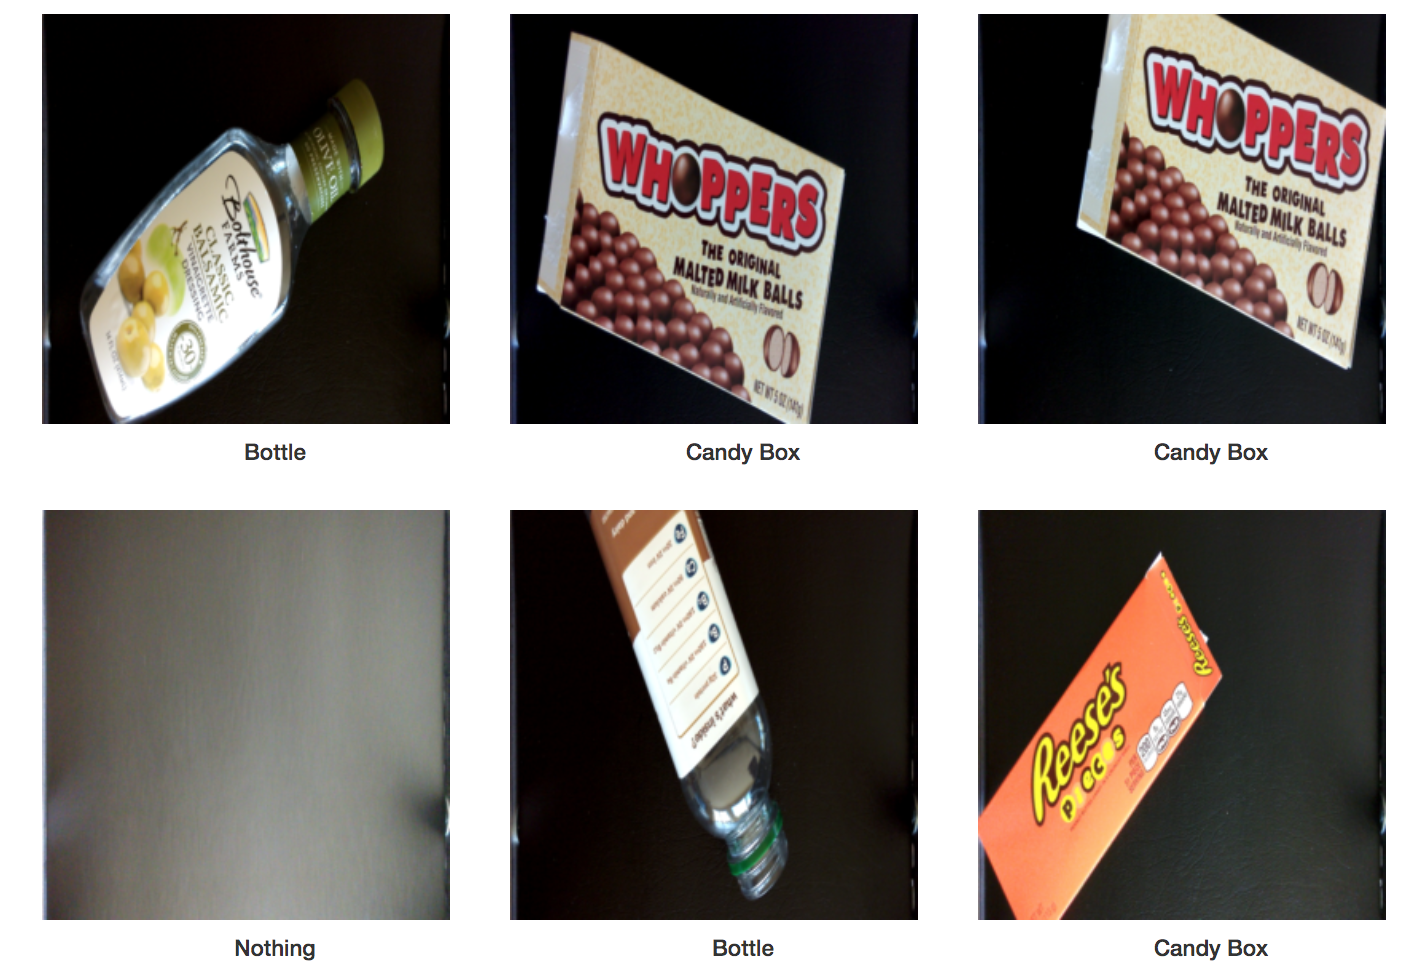
\includegraphics[width=\linewidth]{suplieDataset.png}
      \caption{Supplied Data set.}
      \label{fig:robot1}
\end{figure}

\subsubsection{Supplied Data set}
Udacity supplied data set contain candy boxes, bottles, and nothing. Photos taken from a Jetson mounted over a conveyor belt. By training pictures of candy boxes, bottles, and nothing (empty conveyor belt) for the purpose of real time sorting. This kind of design can be extrapolated to many things that require real time sorting.

\section{Background / Formulation}

These example images come from a combination of the GTI vehicle image database, the KITTI vision benchmark suite, and examples extracted from the project video itself. Penn-Fudan Database for Pedestrian Detection and Segmentation.

 The intuition is from:
 %example for Bullet point list

\begin{itemize}
\item Can you form a model that can tell the difference between cars or not cars?
\item Can you form a model that can tell the difference between Pedestrian and cars?
\end {itemize}
 %example for inserting image
\begin{figure}[thpb]
      \centering
      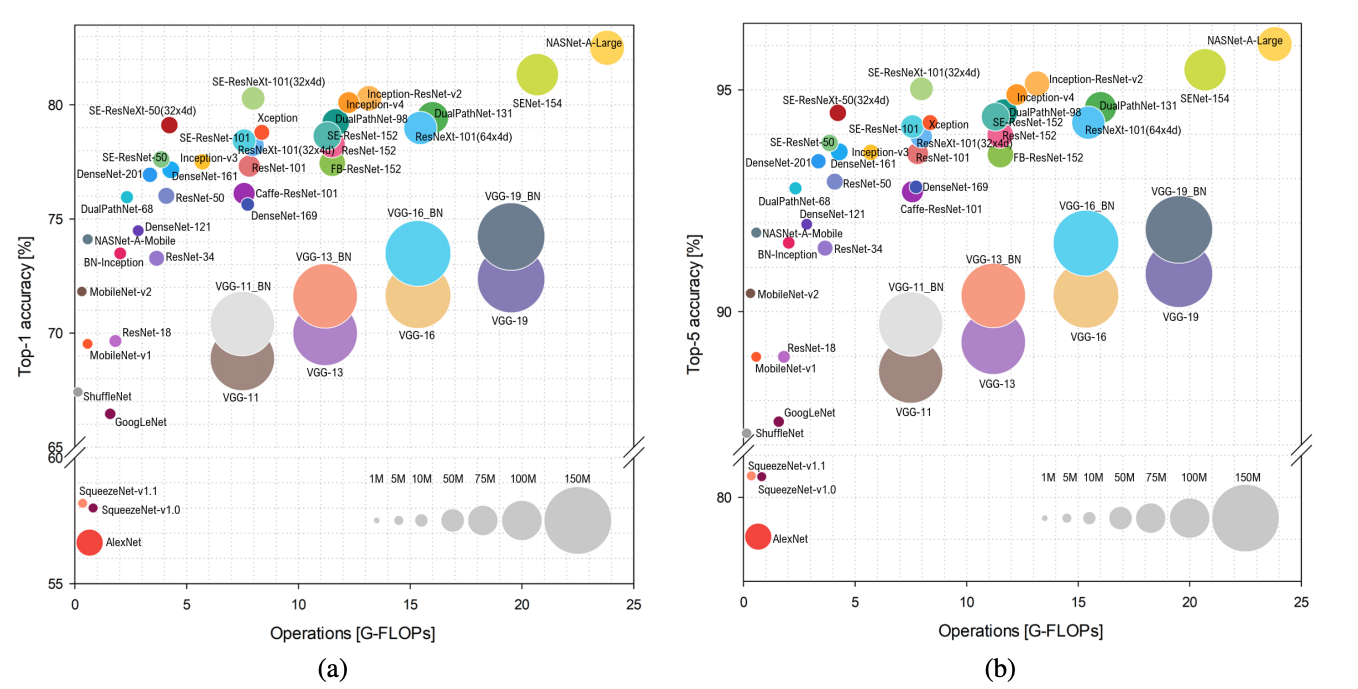
\includegraphics[width=\linewidth]{BenchmarkAnalysisofRepresentativeDeep NeuralNetworkArchitectures.png}
      \caption{Benchmark Analysis of Representative
Deep Neural Network Architectures [9].}
      \label{fig:robot1}
\end{figure}
 Compare to different Neural Network architecture(see Fig. 2)and
 accuracy. VGG16 pretrained model, AlexNet and GoogLeNet seems to be a good choice.
\section{Data Acquisition}
Udacity supplied data set contain 3 classes Bottle, candy box and nothing.
\begin{table}[h]
 \begin{center}
      \begin{tabular}{ |c|c|c| } 
       \hline
       Class & Images & Image Shape \\
       \hline
       Candy Box & 1871 & 256x256x3 \\ 
       Bottle & 3426 & 256x256x3 \\ 
       Nothing & 2273 & 256x256x3 \\
       \hline
       Total & 7570 & \\
       \hline
      \end{tabular}
      \caption{Count of supplied data images}
      \label{table:1}
      \end{center}
      \end{table}
The combination of public data set is collect from Udacity Self-Driving car Engineer Vehicle detection project[6] and Penn-Fudan Database for Pedestrian Detection and Segmentation [7].
%example for inserting image
\begin{figure}[thpb]
      \centering
      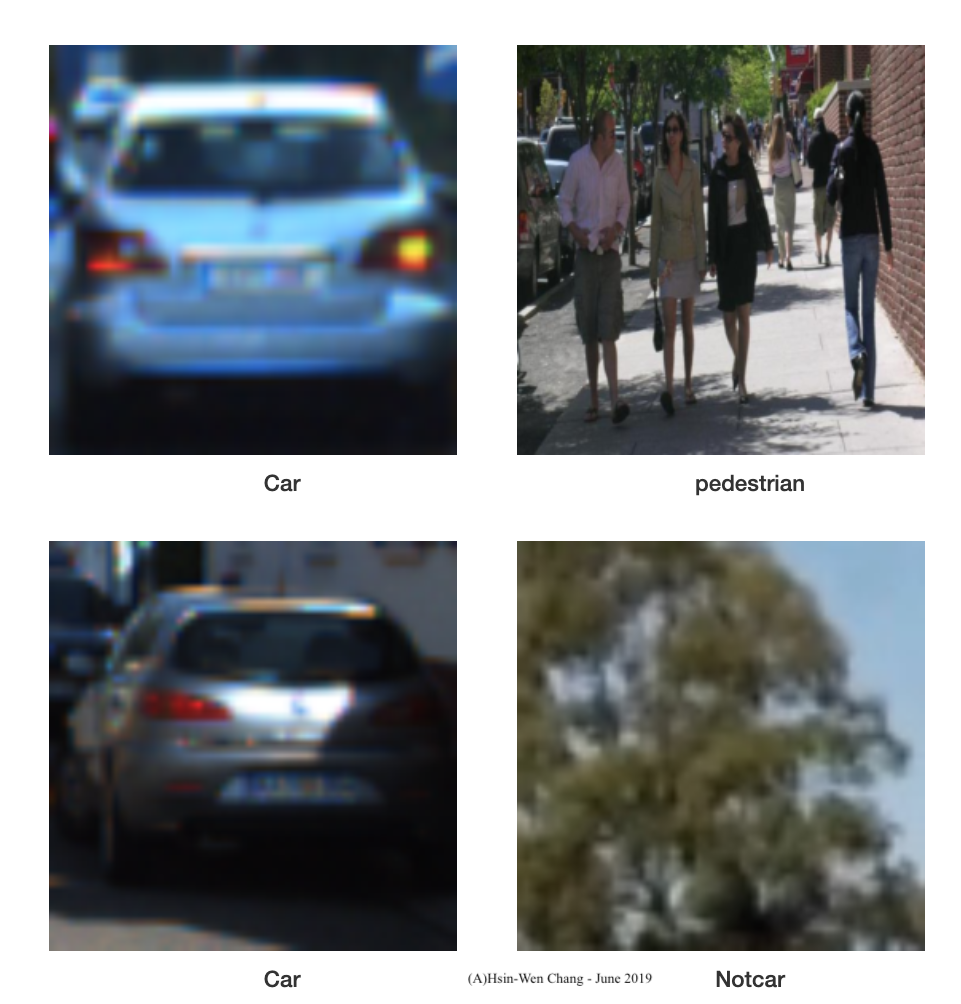
\includegraphics[width=\linewidth]{mixDataset.png}
      \caption{Combination data set.}
      \label{fig:robot1}
\end{figure}

\section{Results-}
In this section, we will discuss the result as two part. The training result on Udacity supplide data set and on the mixed public data set from Penn-Fudan Database for Pedestrian Detection and Segmentation and the GTI vehicle image database, the KITTI vision benchmark suite, and examples extracted from the Udacity Self-Driving car Engineer Vehicle detection project [6] video itself. Supplied data set was used on test VGG16 pretrained model and AlexNet. Acurracy of VGG16 pretrained model is really close to near 100 percent slightly higher than AlexNet which accuracy is close to 96-97 percent when applied 50 epochs. After test on supplied data set as reference, then we choose GoogLeNet to train on our mixed public data set. The accuracy is higher than AlexNet when using 50 epochs same as reference paper [10]. Result are show in figure 4-11.
%example for inserting image
\begin{figure}[thpb]
      \centering
      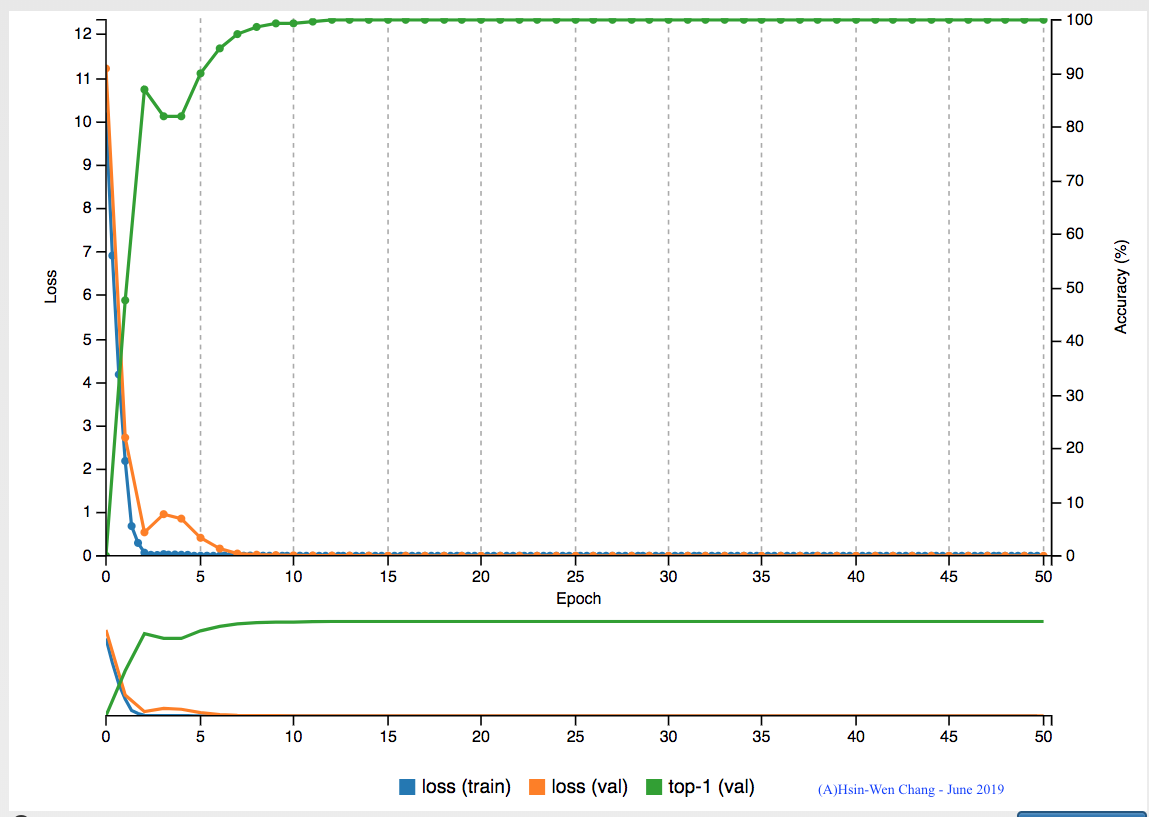
\includegraphics[width=\linewidth]{VGG16AcurracyLoss.png}
      \caption{VGG16 pretrained model}
      \label{fig:robot1}
\end{figure}
\begin{figure}[thpb]
      \centering
      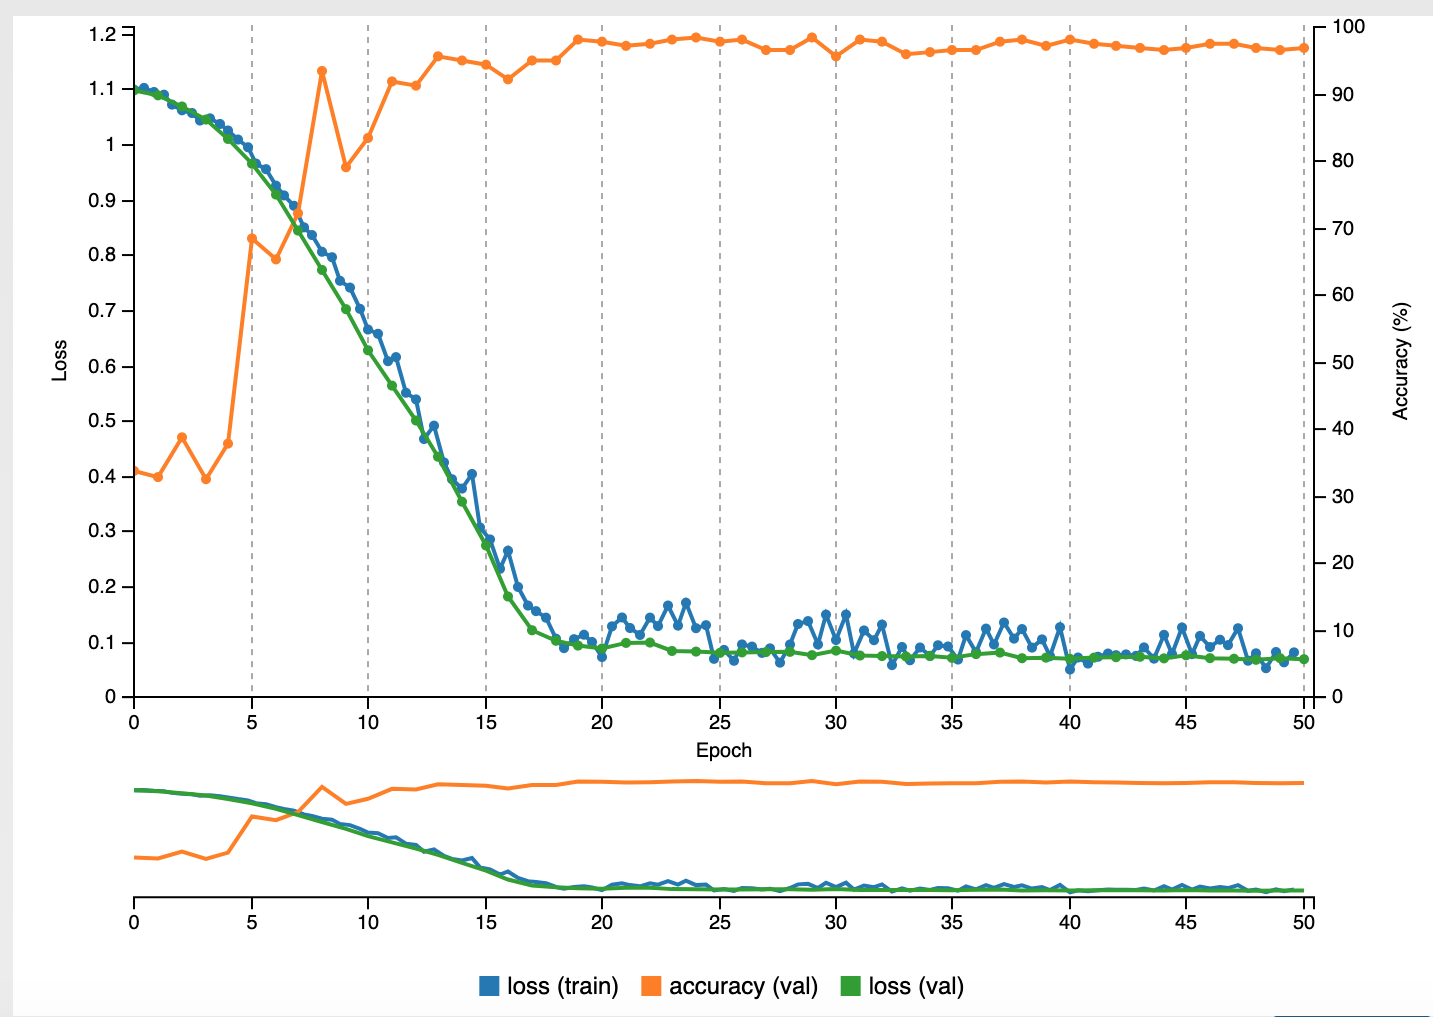
\includegraphics[width=\linewidth]{AlexNet.png}
      \caption{AlexNet}
      \label{fig:robot1}
\end{figure}
%example for inserting image
\begin{figure}[thpb]
      \centering
      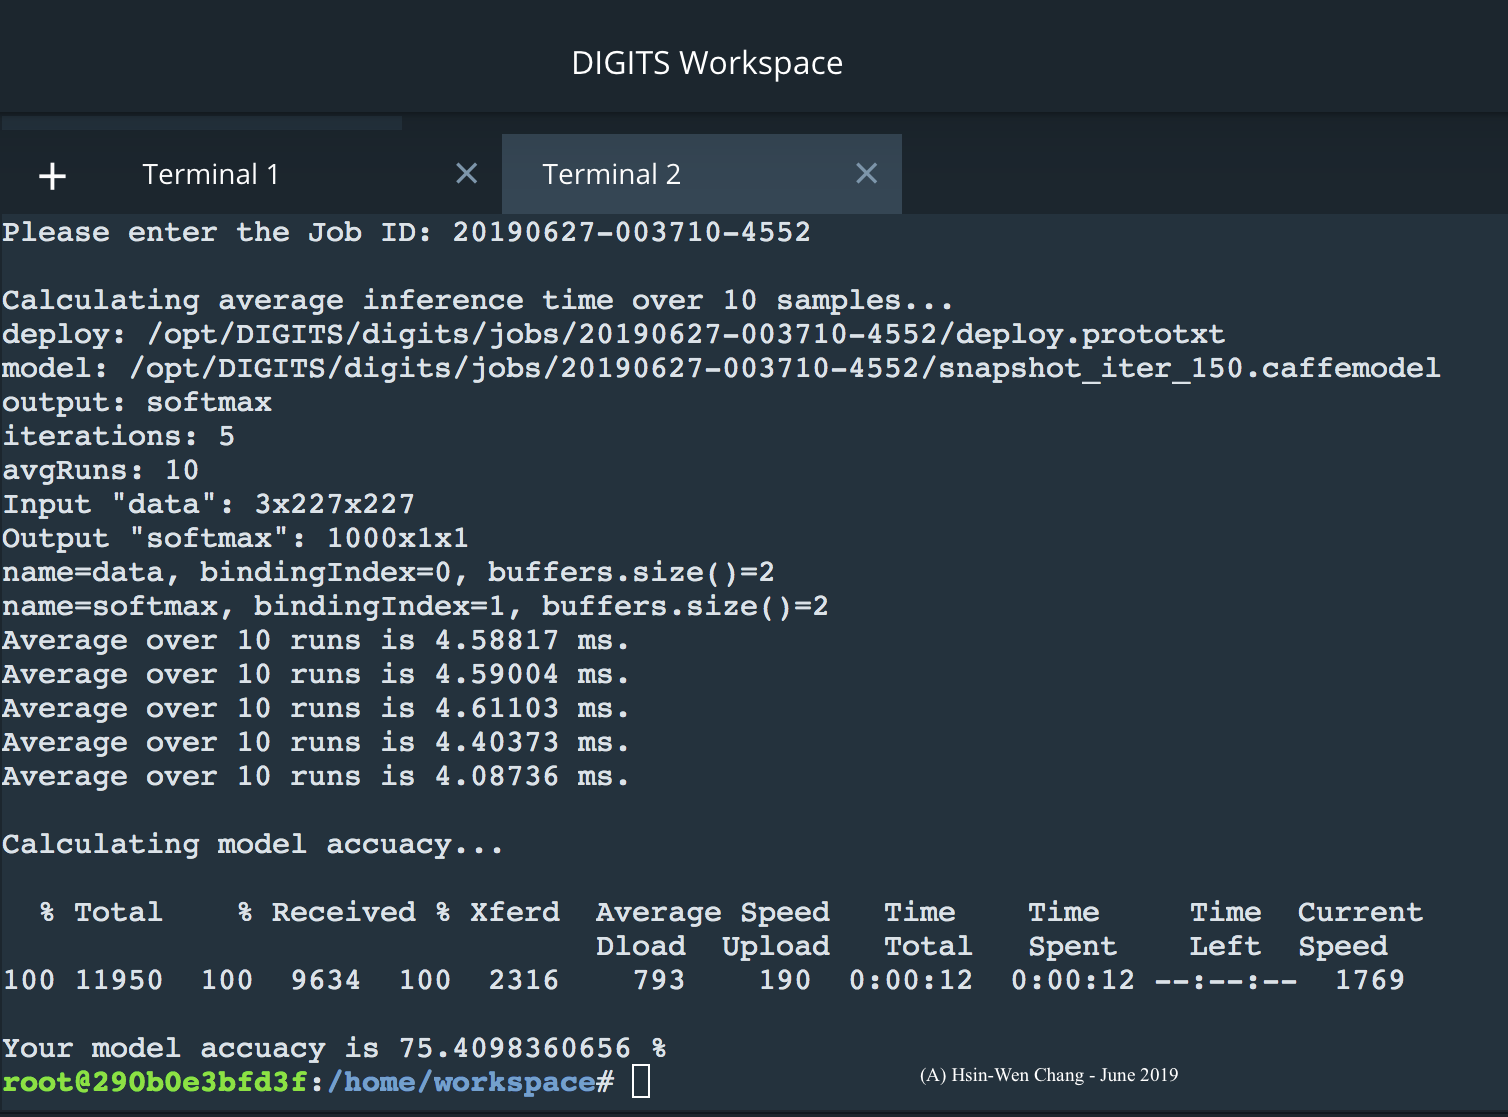
\includegraphics[width=\linewidth]{evaluate.png}
      \caption{Evaluate training result in DIGITS Workspace}
      \label{fig:robot1}
\end{figure}
%example for inserting image
\begin{figure}[thpb]
      \centering
      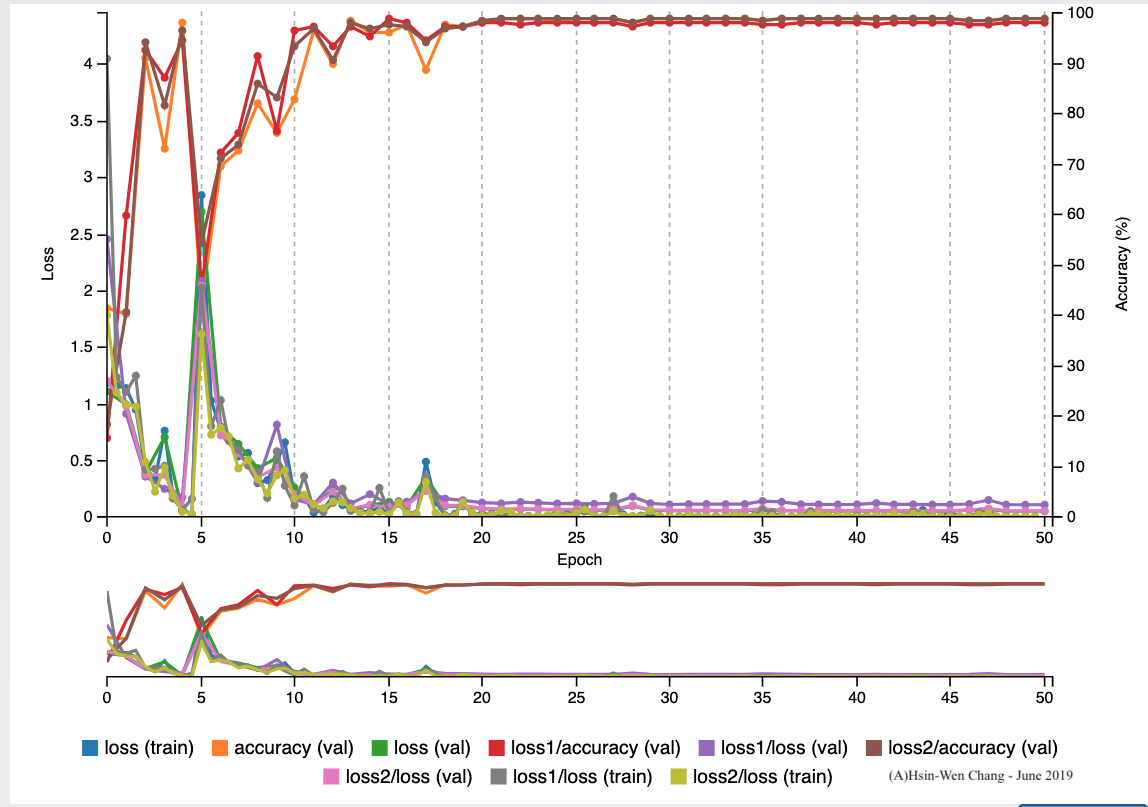
\includegraphics[width=\linewidth]{GoogLeNET.png}
      \caption{Combination data train with GoogLeNet}
      \label{fig:robot1}
\end{figure}
\begin{figure}[thpb]
      \centering
      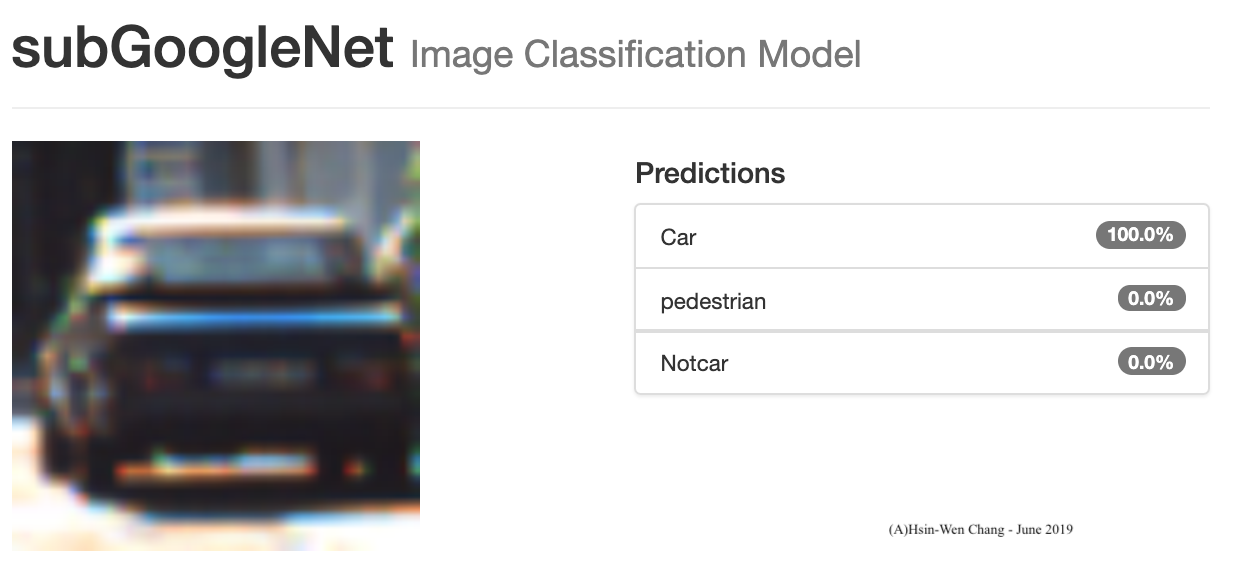
\includegraphics[width=\linewidth]{CarInferenceResult.png}
      \caption{GoogLeNet Model Inference Result: Car}
      \label{fig:robot1}
\end{figure}
\begin{figure}[thpb]
      \centering
      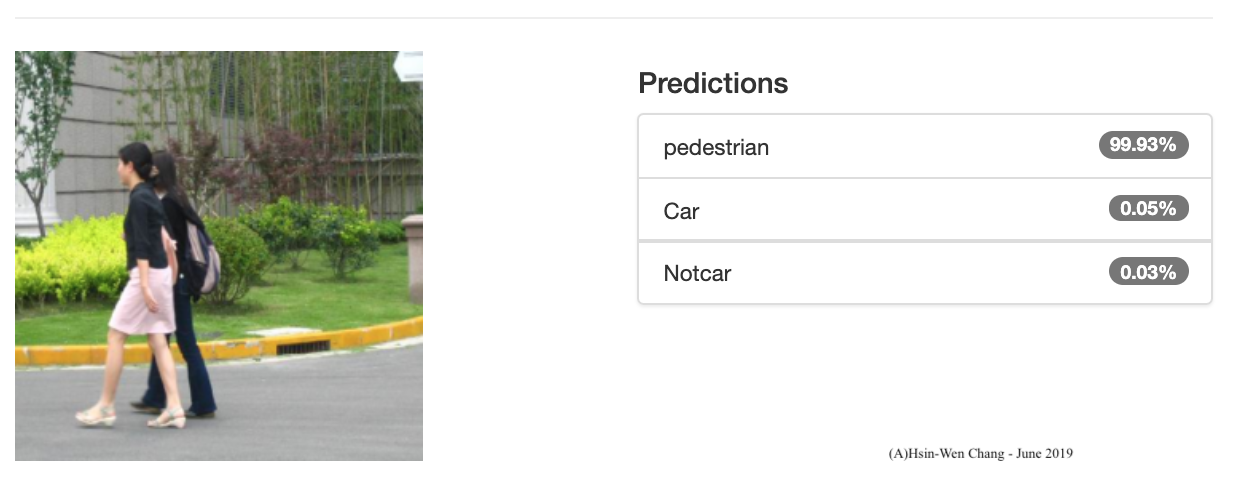
\includegraphics[width=\linewidth]{GoogLenetPed.png}
      \caption{GoogLeNet Model Inference Result: Pedestrian}
      \label{fig:robot1}
\end{figure}
\begin{figure}[thpb]
      \centering
      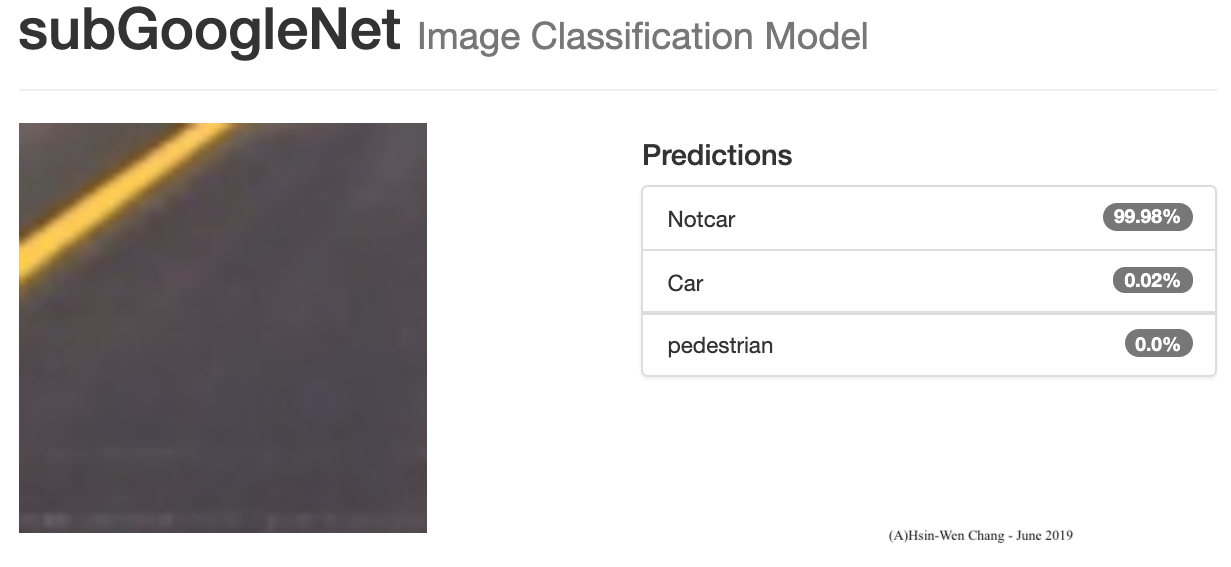
\includegraphics[width=\linewidth]{notCarInferenceGoodResult.png}
      \caption{GoogLeNet Model Inference Result: Not Car}
      \label{fig:robot1}
\end{figure}
\begin{figure}[thpb]
      \centering
      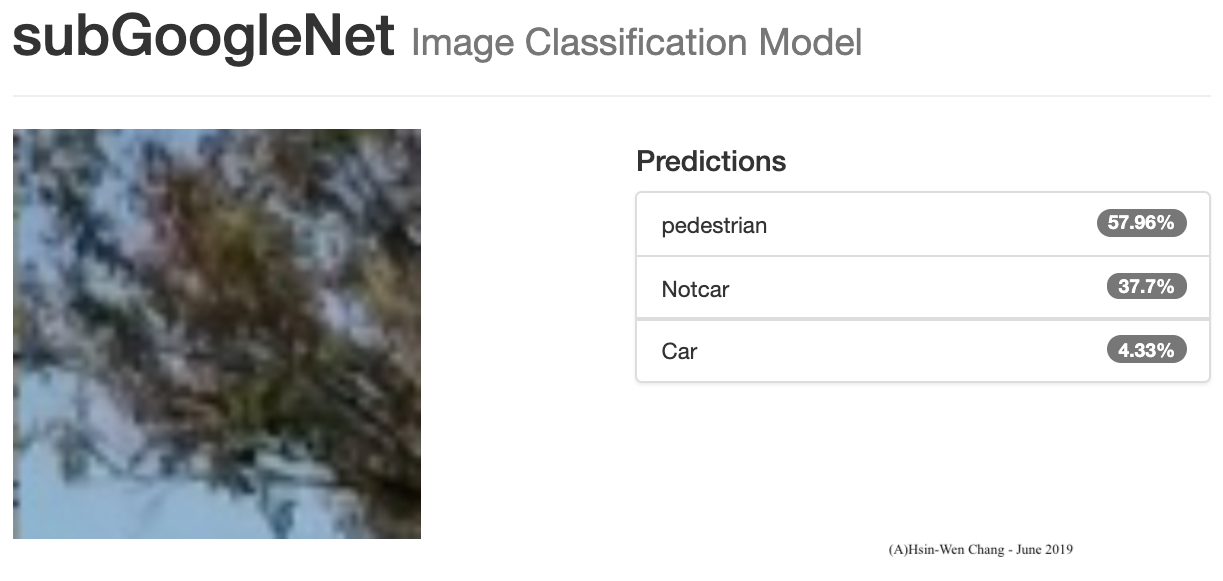
\includegraphics[width=\linewidth]{NotCarInference.png}
      \caption{GoogLeNet Model Inference Result: Not Car}
      \label{fig:robot1}
\end{figure}


\section{Discussion}
There is a slightly improvement when switch model from AlexNet to GoogLeNet while GoogLeNet need more time to train and perform inference results. We can use improved hardware like Jetson TX2 and Tensor RT 3.0 to improve performance in a very fast time.

\section{Conclusion / Future work}
GoogLeNet have better accuracy for sensor like camera and video on perform image classification task on detect pedestrian, car and their background environment with higher accuracy than AlexNet but will cost longer time to inference results and training images. Base on the research and studying in Udacity Self-Driving Car Engineer Nanodegree - Semantic Segmentation Project [9], the inference time to perform real-time computer vision is crucial hence in the future work we can apply transfer learning skill on VGG16 for less inference time and higher accuracy. Another way to improve accuracy base on our current model we can add more image data but this will prolong training time and cost more storage space.

\bibliography{bib}
\bibliographystyle{ieeetr}

[1] The Caltech Database (Computational Vision at California Institute of Technology, Pasadena), http://www.vision.caltech.edu/html-files/archive.html. Accessed 14 May 2011.

[2] R Fergus, P Perona, A Zisserman, in Proceedings of the IEEE Computer Society Conference on Computer Vision and Pattern Recognition, Madison, Wisconsin, 16–22 June 2003.

[3] The TU Graz-02 Database (Graz University of Technology). Accessed 14 May 2011. 

[4] A Opelt, A Pinz, in Proceedings of the 14th Scandinavian Conference on Image Analysis, Joensuu, Finland, 19–22 June 2005.

[5] Are we ready for Autonomous Driving? The KITTI Vision Benchmark Suite, Andreas Geiger, Philip Lenz and Raquel Urtasun, Conference on Computer Vision and Pattern	Recognition (CVPR).

[6] Udacity Self-Driving car Engineer Vehicle detection project.

[7] Object Detection Combining Recognition and Segmentation. Liming Wang, Jianbo Shi, Gang Song, I-fan Shen. To Appear in ACCV 2007.

[8] Udacity Self-Driving Car Engineer Nanodegree - Semantic Segmentation Project.

[9] Benchmark Analysis of Representative Deep Neural Network Architectures. SIMONE BIANCO1,REMI CADENE2,LUIGI CELONA1 AND PAOLO NAPOLETANO,https://arxiv.org/pdf/1810.00736.pdf,ACCESS.2017.
\end{document}